\documentclass[12pt]{article}

\usepackage{graphicx} % Allows including images
\usepackage{booktabs} % Allows the use of \toprule, \midrule and \bottomrule in tables
\usepackage{amsmath}
\usepackage{amsfonts}
\usepackage{ifthen}
\usepackage{amssymb}
\usepackage{amsbsy}
\usepackage{bm}
\usepackage{ulem}
\usepackage{float}
\usepackage{latexsym}
\usepackage{comment}
\usepackage{graphicx}
\usepackage{amstext}
\usepackage{latexsym}
\usepackage{arydshln}
\usepackage{longtable}
\usepackage{enumerate}
\usepackage{multirow}
\usepackage{cases}
\usepackage{geometry}
\usepackage{mathtools}
\usepackage{subeqnarray}
\usepackage{textcomp}
\usepackage{hyperref}
%\usepackage{subfigure}
\usepackage{url}
\usepackage{threeparttable}
\usepackage{xr}
\usepackage{multirow}
\usepackage{wrapfig}
\usepackage{lscape}
\usepackage{rotating}
\usepackage{subcaption}
\usepackage{epstopdf}
\usepackage{verbatim}
\usepackage{xcolor}
\usepackage[sort&compress]{natbib}
\usepackage{bm}


\captionsetup{font={small}}
\geometry{left=1.0cm, right=1.0cm, top=1.0cm, bottom=1.0cm}

\title{EE526 Homework 1}

\author{Xingche Guo}

\date{\today}

\linespread{1.3}
\begin{document}
\maketitle

%%%%%%%%%%%%%%%%%%%%%%
\centering

\section*{Problem 1}

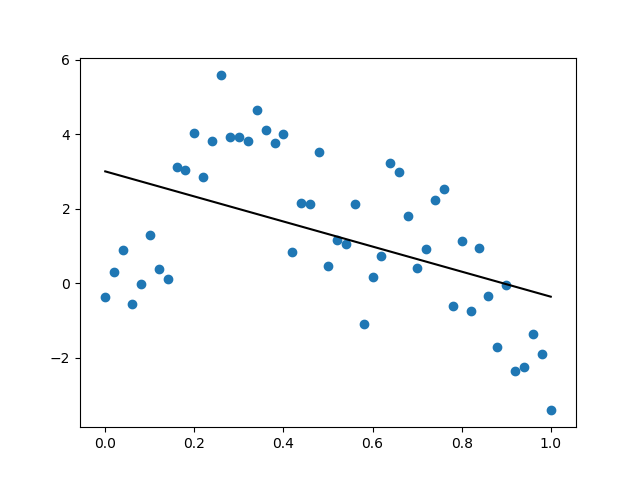
\includegraphics[width = 0.4\textwidth]{fig1_0.png}
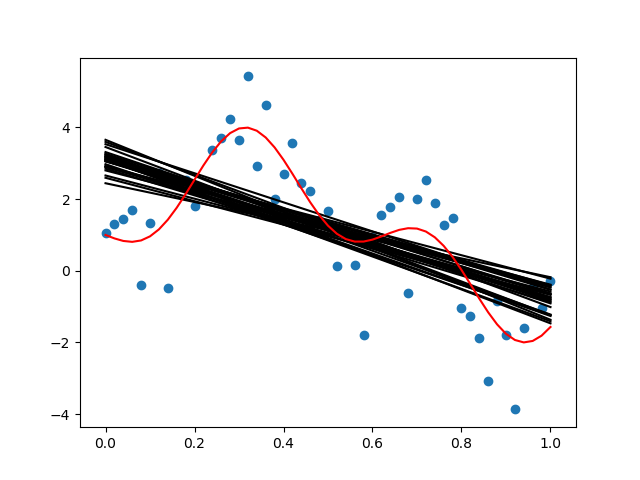
\includegraphics[width=.4\linewidth]{fig1.png}
 
 
 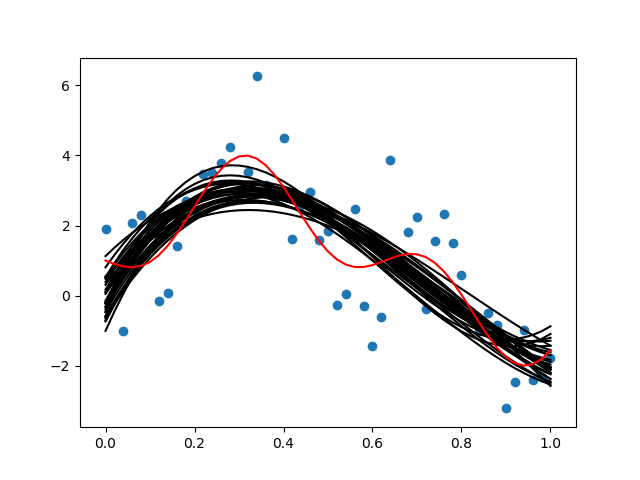
\includegraphics[width=.4\linewidth]{fig3.png}
 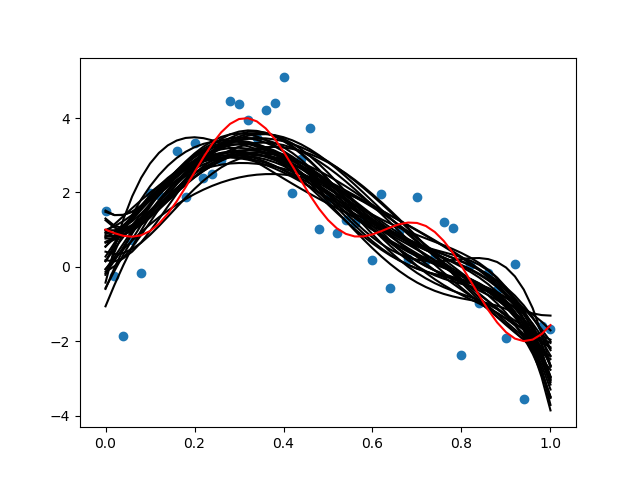
\includegraphics[width=.4\linewidth]{fig5.png}
 
 
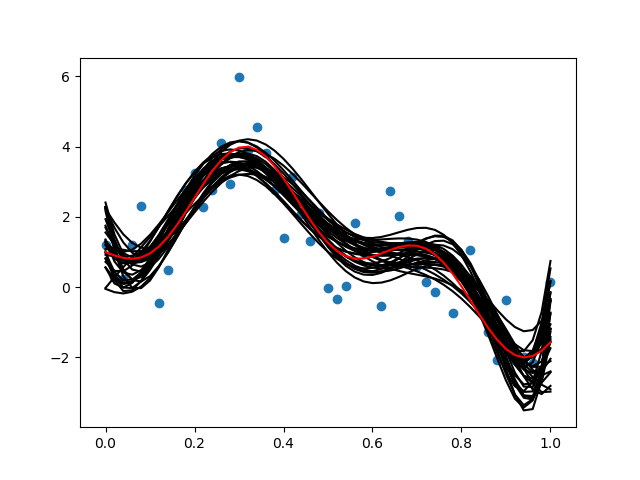
\includegraphics[width=.4\linewidth]{fig7.png}
  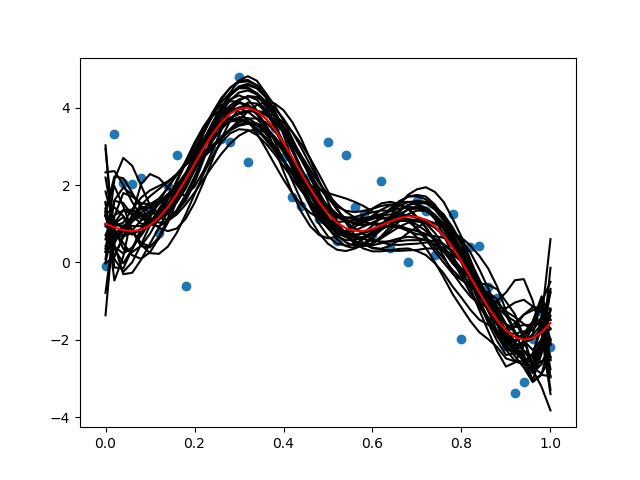
\includegraphics[width=.4\linewidth]{fig9.png}
  
  
 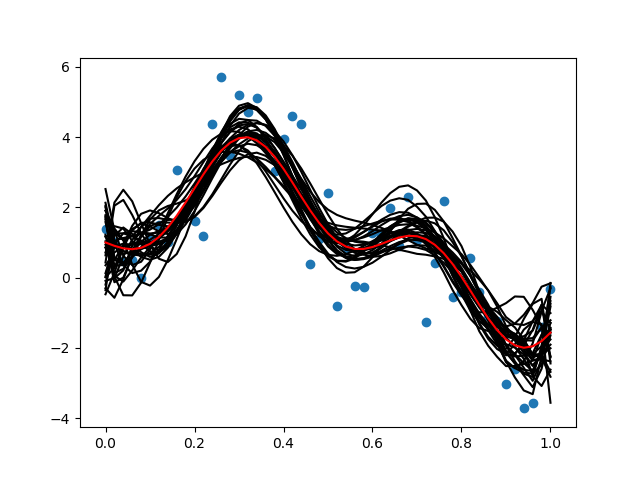
\includegraphics[width=.4\linewidth]{fig11.png}







%%%%%%%%%%%%%%%%%%%%
\section*{Problem 2}

 \begin{figure}[h]
  \centering
  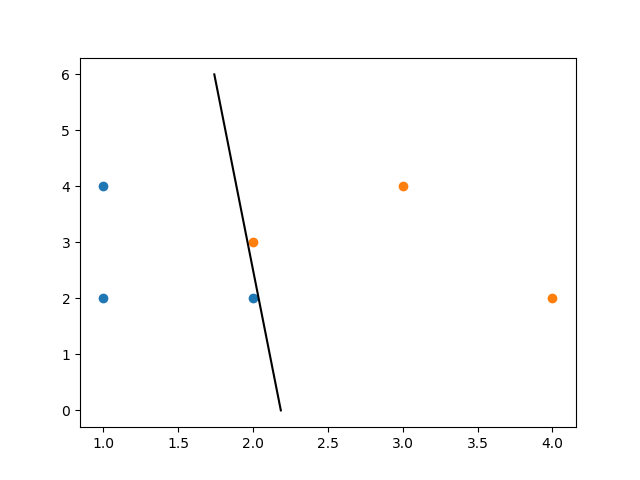
\includegraphics[width = 0.80\textwidth]{perceptron.png}
 \end{figure}	



%%%%%%%%%%%%%%%%%%%%%%
\section*{Problem 3}

Let $\bm{\beta}_0 = (0, \dots, 0)^T$, jump out of the loop if: $ \frac{|| \bm{\beta} - \bm{\beta}_0 ||}{||\bm{\beta}_0|| + \epsilon}$ less than a certain threshold, then:

\begin{tabular}{ |c|ccccccc| } 
\hline
Learning Rate & $10^2$ & $10$  & $1$  & $10^{-1}$  &  $10^{-2}$  &  $10^{-3}$  &  $10^{-4}$  \\
 \hline
 Training Error Rate (unnormalized) & 0.095  & 0.094  & 0.094 & 0.110 & 0.094 & 0.101 & \textcolor{red}{0.145} \\ 
 Training Error Rate (normalized) &  \textcolor{red}{0.087} &  0.049 & 0.052 &  0.055 & 0.062 & 0.076 & 0.082 \\ 
 Testing Error Rate (unnormalized) & 0.190  & 0.188  & 0.188 & 0.188 & 0.188 & 0.184 & \textcolor{red}{0.236} \\ 
 Testing Error Rate (normalized) & \textcolor{red}{0.139}  & 0.132  & 0.124  & 0.122 & 0.131 & 0.148 & 0.157 \\ 
 \hline
\end{tabular}


\textcolor{red}{red number} means obtain the maximum iteration number/the algorithm fail to converge.





\end{document}

















